%!TEX program = Xelatex
\documentclass{article}
%\usepackage{ctex}
\usepackage{amsmath,amscd,amsbsy,amssymb,latexsym,url,bm,amsthm}
\usepackage{epsfig,graphicx,subfigure}
\usepackage{enumitem,balance,mathtools}
\usepackage{wrapfig}
\usepackage{mathrsfs, euscript}
\usepackage[usenames]{xcolor}
\usepackage{hyperref}
\usepackage{caption}
\usepackage{setspace}
%\usepackage{subcaption}
\usepackage{float}
\usepackage{listings}
\usepackage{hyperref}
%\usepackage{enumerate}
%\usepackage{algorithm}
%\usepackage{algorithmic}
%\usepackage[vlined,ruled,commentsnumbered,linesnumbered]{algorithm2e}
\usepackage[ruled,lined,boxed,linesnumbered]{algorithm2e}

\newtheorem{theorem}{Theorem}[section]
\newtheorem{lemma}[theorem]{Lemma}
\newtheorem{proposition}[theorem]{Proposition}
\newtheorem{corollary}[theorem]{Corollary}
\newtheorem{exercise}{Exercise}[section]
\newtheorem*{solution}{Solution}

\renewcommand{\thefootnote}{\fnsymbol{footnote}}
\renewenvironment{solution}[1][Solution]{~\\ \textbf{#1.}}{~\\}
\newcommand{\myblock}[2]{\textbf{#1}\ {#2}}
\newcommand{\postscript}[2]
    {\setlength{\epsfxsize}{#2\hsize}
    \centerline{\epsfbox{#1}}}

\renewcommand{\baselinestretch}{1.0}

\setlength{\oddsidemargin}{-0.365in}
\setlength{\evensidemargin}{-0.365in}
\setlength{\topmargin}{-0.3in}
\setlength{\headheight}{0in}
\setlength{\headsep}{0in}
\setlength{\textheight}{10.1in}
\setlength{\textwidth}{7in}

\title{CS222 Homework 4}
\author{Algorithm Analysis \& Deadline: 2020-11-04 Wednesday 23:59}
\date{Exercises for Algorithm Design and Analysis by Li Jiang, 2020 Autumn Semester}

\begin{document}

\maketitle

\begin{enumerate}
\item
Given a integer set S, which has n elements in it, you need to divide this set into 2 subarray, where the subarray S1 has m elements, and the subarray S2 has (n-m) elements. the target is minimizing $abs(sum(S1) -sum(S2))$.

Implement your algorithm with C/C++/Python. Please attach your source code named as {\color{red}\emph{Code-P1.*}}. The file \texttt{Data-P1.txt} is a test case, includes an 1-D array of integer with random length, and your program needs to output the final sum. You need to briefly describe your algorithm and find the final sum of \texttt{Data-P1.txt} by your program.

\textbf{Example:}

Given input array: $arr[]={1, 6, 11, 5}$. The algorithm should return $1$. The subset $S1=[1, 5, 6], S2=[11]$ .

\begin{solution}
~\\
\myblock{Def.}{}
$$f(i,sum)=\left\{\begin{array}{ll}True\ ,& if\ \exists\ I\subseteq \{1,2,3,\cdots,i\}\ s.t.\ \sum_{j\in I} S_j = sum\\False\ ,& otherwise \end{array}\right.$$
\myblock{Recursion:}{} 
$$f(i+1,sum) = f(i,sum) \vee f(i, sum-S_i)$$
\myblock{Initialization:}{}
$$f(0, 0) = True$$
Traverse $f(n, s)$ to check whether $S$ can be divide to two parts $S_1$ and $S_2$ s.t. $Sum(S_1)=s$.\\
With proper recursion order, the component $i$ is not necessary. We can finish it in $\Theta(nS)$ \textbf{time} and $\Theta(S)$ \textbf{space}.\\
~\\
\textbf{Result of my program on test data}: 1\\
\href{run:./code/main1.cpp}{\textbf{Code for P1}}: read from "./code/Data-P1.txt", and print the minimal $|sum_1-sum_2|$ to the screen. It is recommended to turn on the '-O2' option. It takes about $30s$ to run the example test data on my computer. I used fixed length array, so the test data's length should not be larger than $1000000$.
\end{solution}

~\\
~\\
    \item 
    \textbf{Bookshelf: }Tim has $n$ books and he wants to make a bookshelf to them. The pages' width of the $i$-th book is $w_i$ and the thickness is $t_i$. 

    Tim puts the books on the bookshelf in the following way. He selects some books and put them vertically. Then the rest of the books are put horizontally above the vertical books. Obviously, the total thickness of the books put vertically must be greater than the sum of widths of the horizontal books. As long as tim wants to make the bookshelf as small as possible, please help him to find the minimum total thickness of the vertical books.

    To simplify the problem, the thickness of each book is either $1$ or $2$. And all the numbers in this problem are positive integers.

    Design an algorithm based on dynamic programming and implement it in C/C++/Python. The file \texttt{Data-P2.txt} is a test case, where the first line contains an integer $n$. Each of the next $n$ lines contains two integers $t_i$ and $w_i$ denoting two attributes of the $i$-th book. Source code should be named as
    {\color{red}\emph{Code-P2.*}} .You need to briefly describe your algorithm and find the result of \texttt{Data-P2.txt} by your program.

    \textbf{Example:}

    Given $n=5$ books, and $\{(t_i,w_i)|1\leq i \leq 5\} = \{(1,12),(1,3),(2,15),(2,5),(2,1)\}$. The algorithm should return $5$.

    \begin{solution}
    ~\\
    \myblock{Def.}{$f(i, t) :=$ the minimal width $w$ of books when the thickness is exactly $t$.} i.e. $$f(i,t):=\min_{S\subseteq\{1,2,\cdots,i\}} \sum_{i\in S} w_i\ ,\ s.t. \sum_{i\in\{1,2,\cdots,i\}\setminus S} t_i = t$$
    \myblock{Recursion:}{$$f(i, t) = \min\{f(i-1, t-t_i), f(i-1, t)+w_i\}$$}
    For the $i-th$ book, there are two options:\begin{itemize} \item [1)] Put vertically, then the optimal value is $f(i-1, t-t_i)$. \item [2)] Put horizontally, then the optimal value is $f(i-1,t)+w_i$.\end{itemize} 
    \myblock{Initialization:}{$$f(0,t)=\left\{\begin{array}{ll}0, &if\ t=0\\+\infty, &otherwise\end{array}\right.$$}
    The thickness $t$ is feasible if and only if $f(n, t) \leq t$. So after calculate $f(.)$, we only need to find $$\min t\,\ s.t.\ f(n,t)\leq t$$
    With proper recursion order, the component $i$ is not necessary. \textbf{Time} $O(n^2t_{max})$, \textbf{Space:} $O(nt_{max})$.\\
    \myblock{Result of my program on test data:}{2542}\\
    \href{run:./code/main2.cpp}{\textbf{Code for P2}}: read from "./code/Data-P2.txt", and print the minimal thickness to the screen. It is recommended to turn on the '-O2' option. It takes less than $1s$ to run the example test data on my computer.
    \end{solution}

~\\
~\\

    \item
    Recall the \emph{String Similarity} problem in class, in which we calculate the edit distance between two strings in a sequence alignment manner.

    You are to find the lowest aligning cost between 2 DNA sequences, in which the cost matrix is defined as

    \begin{center}
        \begin{tabular}{|c||c|c|c|c|c|}
        \hline
          & - & A & T & G & C \\
        \hline
        - & 0 & 1 & 2 & 1 & 3 \\
        A & 1 & 0 & 1 & 5 & 1 \\
        T & 2 & 1 & 0 & 9 & 1 \\
        G & 1 & 5 & 9 & 0 & 1 \\
        C & 3 & 1 & 1 & 1 & 0 \\
        \hline
        \end{tabular}
    \end{center}

    where \texttt{(-, A)} means adding (or removing) one \texttt{A}, etc.

    \begin{enumerate}
        \item
        Implement Hirschberg's algorithm with C/C++/Python. Please attach your source code named as {\color{red}\emph{Code-P3.*}}. Your program will be tested against random inputs. Your program should be able to output two sequences after editing.

        \item
        Using your program, find the edit distance between the two DNA sequences found in attachments \texttt{Data-P3a.txt} and \texttt{Data-P3b.txt}.
    \end{enumerate}
\begin{solution}\\
\myblock{Def.}{$f(i,j) := $ the minimal aligning cost between $s_{1\cdots i}$ and $t_{1\cdots j}$, where $s$ and $t$ are the two strings.}\\
\myblock{Recursion:}{\begin{spacing}{1.2}$$f(i, j) = \min\left\{\begin{array}{l}f(i-1,j)+cost(s_i,-)\\f(i,j-1)+cost(-,t_j)\\f(i-1,j-1)+cost(s_i,t_j)\\\end{array}\right.$$\end{spacing}}
\textbf{Time:} $\Theta(length_s\cdot length_t)$ acceptable. \textbf{Space:} $\Theta(length_s\cdot length_t)$ (to record the optimal path) \textbf{not} acceptable.\\
Use the divide and conquer algorithm talked in the class:\\
\begin{figure}[H]
\centering
\caption{Skecth for problem 3}
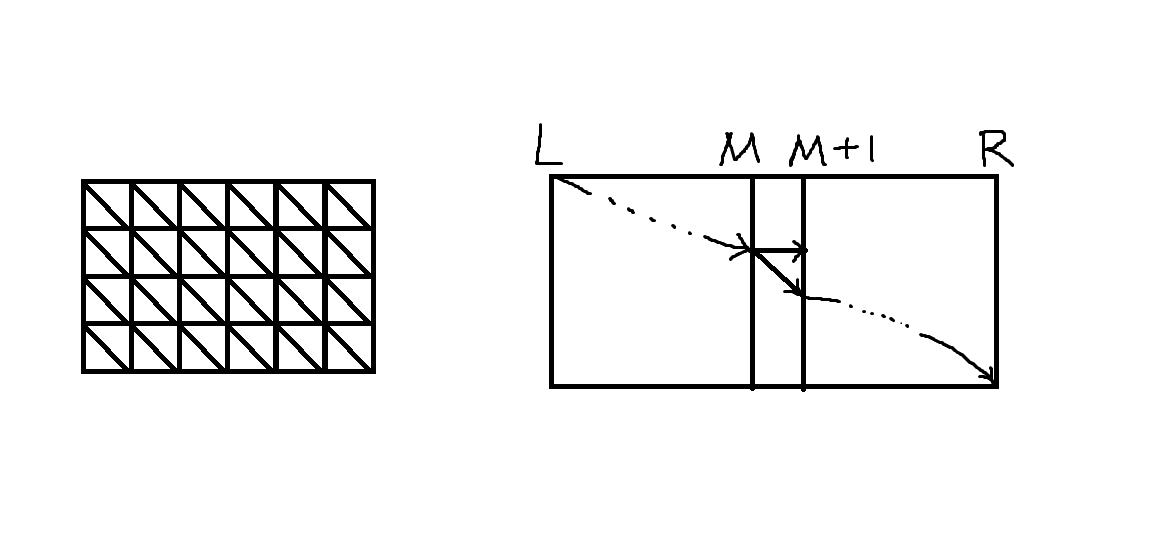
\includegraphics[width=0.8\textwidth]{problem3.png}
\end{figure}
Abstract the origin problem to a shortest path problem on a grid. When $R-L\leq 2$, divide the problem to 2 subproblems. Find the shortest length of path from $(L, top)$ to $(M, *)$, and the shortest length of path from $(M+1,*)$ to $(R,bottom)$, and determine which point is on the shortest path. In the class, we have proved that this algorithm can solve the problem within $\Theta(length_s\cdot length_t)$ \textbf{time} and $\Theta(length_s+length_t)$ \textbf{space}, acceptable.\\
\href{run:./code/main3.cpp}{\textbf{Code for P3}}: read from "./code/Data-P3a.txt" and "./code/Data-P3b.txt", write the result $s'$ to "./code/Data-P3-out-a.txt" and $t'$ to "./code/Data-P3-out-b.txt". And print the minimal edit distance to the screen. It is recommended to turn on the '-O2' option. It takes about $40s$ to run the example test data on my computer. I used fixed length arrays, so the test data should no longer than $1000000$ letters. If you want to test larger data, you should modify the 'MAXN' value in my code.
\end{solution}
~\\
\item
    Considering you are playing a game with your friend, there are n coins placed in one row with the value of v1, v2, ..., vn, respectively. You and your friend can take one coin from row head or row tail sequentially. If you are the first to choose the coin, write an algorithm to ensure that you can get the maximum profit. Suppose that your friend is as smart as you. 
    ~\\
    Implement your algorithm with C/C++/Python. Please attach your souce code named as {\color{red}\emph{Code-P4.*}}. The file \texttt{Data-P4.txt} is a test case, includes an 1-D array of unsigned integer with random length, and your program needs to output the the coin value list that you choose, and the maximum profit you will get. You need to briefly describe your algorithm and find the final answer of \texttt{Data-P4.txt} by your program.
    
    textbf{Example:}

    Given input array: $arr[]={8, 15, 3, 7}$. The algorithm should return your choice list [7, 15], and the final profit 22. 
    
    \begin{solution}~\\
    Game problem. Max-min. Your policy is to maximize the estimated value of the game state, while the other play's policy is to minimize the estimated value of the game state. The estimated value of the game state is defined from your point of view:\\~\\
    \myblock{Def.}{$f(i,j) :=$ the maximum profit you can get from the sequence $(v_i,v_{i+1},\cdots,v_{j})$ if you play first.}\\
    \myblock{Equation:}{$$f(i,j) = \left\{\begin{array}{ll}v_i, & if\ i=j\\ \max\{v_i,v_j\}, & if\ i+1=j\\\max\{v_i+\min\{f(i+2,j), f(i+1,j-1)\}, v_j+\min\{f(i,j-2), f(i+1,j-1)\}\}, & if\ i+1<j \end{array}\right.$$}
    If $i+1<j$, then there are two choices for you:\begin{itemize}
        \item [1)] Take one from row head: you get $v_i$. Then the other player will take an action to minimize your left profit. So your profit is $v_i+\min\{f(i+2,j), f(i+1,j-1)\}$
        \item [2)] Take one from row tail: you get $v_j$. Then the other player will take an action to minimize your left profit. So your profit is $v_j+\min\{f(i,j-2), f(i+1,j-1)\}$
    \end{itemize}
    Your maximum profit is the larger one of the two choices above.\\
    \myblock{Result of my program on test data:}{250072}\\
    \href{run:./code/main4.cpp}{\textbf{Code for P4}}: read from "./code/Data-P4.txt" and write the answer (both the optimal step and value) to the file "./code/Data-P4-out.txt". It is recommended to turn on '-O2' option. The length of test data should be no larger than  100000. If you do want to test larger data, you should modify 'MAXN' value in my code.
    \end{solution}

~\\
~\\


\textbf{Remark}: You need to upload your .pdf file and write the pseudocode.
\end{enumerate}

\end{document}
